\chapter{Arhitektura i dizajn sustava}
		
		\textbf{\textit{dio 1. revizije}}\\

		\textit{ Potrebno je opisati stil arhitekture te identificirati: podsustave, preslikavanje na radnu platformu, spremišta podataka, mrežne protokole, globalni upravljački tok i sklopovsko-programske zahtjeve. Po točkama razraditi i popratiti odgovarajućim skicama:}
	\begin{itemize}
		\item 	\textit{izbor arhitekture temeljem principa oblikovanja pokazanih na predavanjima (objasniti zašto ste baš odabrali takvu arhitekturu)}
		\item 	\textit{organizaciju sustava s najviše razine apstrakcije (npr. klijent-poslužitelj, baza podataka, datotečni sustav, grafičko sučelje)}
		\item 	\textit{organizaciju aplikacije (npr. slojevi frontend i backend, MVC arhitektura) }		
	\end{itemize}

	
		

		

				
		\section{Baza podataka}
			
			\textbf{\textit{dio 1. revizije}}\\
			
		\textit{Potrebno je opisati koju vrstu i implementaciju baze podataka ste odabrali, glavne komponente od kojih se sastoji i slično.}
		
			\subsection{Opis tablica}
			

				\textit{Svaku tablicu je potrebno opisati po zadanom predlošku. Lijevo se nalazi točno ime varijable u bazi podataka, u sredini se nalazi tip podataka, a desno se nalazi opis varijable. Svjetlozelenom bojom označite primarni ključ. Svjetlo plavom označite strani ključ}
				
				
				\begin{longtblr}[
					label=none,
					entry=none
					]{
						width = \textwidth,
						colspec={|X[6,l]|X[6, l]|X[20, l]|}, 
						rowhead = 1,
					} %definicija širine tablice, širine stupaca, poravnanje i broja redaka naslova tablice
					\hline \SetCell[c=3]{c}{\textbf{korisnik - ime tablice}}	 \\ \hline[3pt]
					\SetCell{LightGreen}IDKorisnik & INT	&  	Lorem ipsum dolor sit amet, consectetur adipiscing elit, sed do eiusmod  	\\ \hline
					korisnickoIme	& VARCHAR &   	\\ \hline 
					email & VARCHAR &   \\ \hline 
					ime & VARCHAR	&  		\\ \hline 
					\SetCell{LightBlue} primjer	& VARCHAR &   	\\ \hline 
				\end{longtblr}
				
				
			
			\subsection{Dijagram baze podataka}
				\textit{ U ovom potpoglavlju potrebno je umetnuti dijagram baze podataka. Primarni i strani ključevi moraju biti označeni, a tablice povezane. Bazu podataka je potrebno normalizirati. Podsjetite se kolegija "Baze podataka".}
			
			\eject
			
			
		\section{Dijagram razreda} 
			
			{ Na slikama su prikazani razredi („Class“) koji su korišteni za implementaciju backend-a. Na slici \ref{fig:controllers} su prikazani razredi koji nasljeđuju Controller razred. Sve funkcije implementirane u Controller razredu vraćaju IActionResult (podatke i odgovarajući kod). Također, sve funkcije ne komuniciraju direktno s bazom podataka nego pozivaju funkcije iz određenih servisa koji imaju implementiranu tu funkcionalnost. Funkcije u kontrolerima kao parametre primaju odgovarajući model. }
			
			\begin{figure}[h]
				\centering
				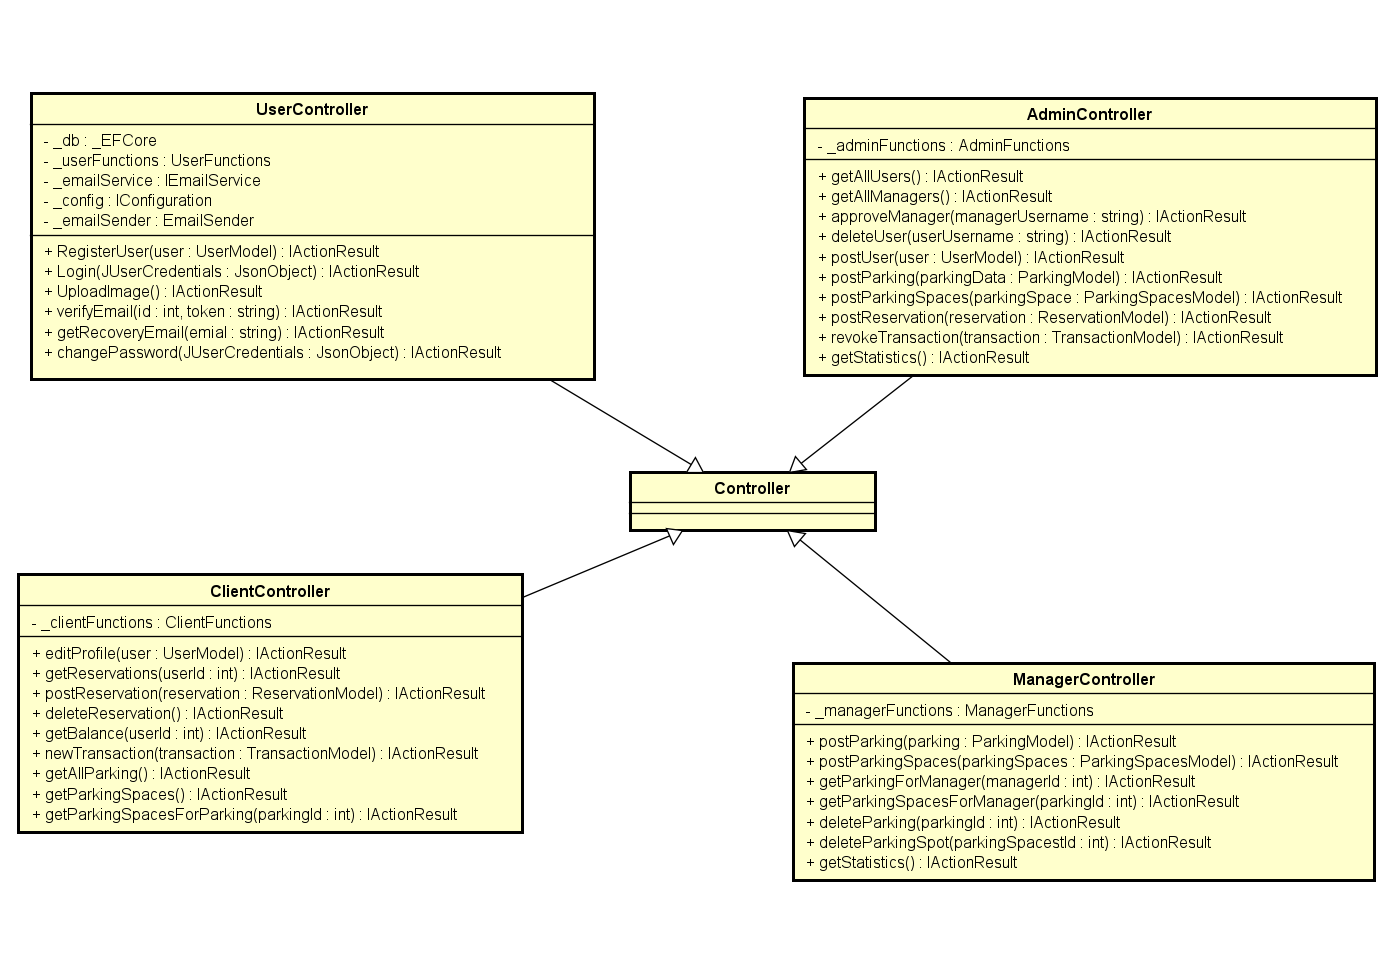
\includegraphics[width=\textwidth,keepaspectratio]{slike/progi4_1.png}
				\caption{dio Controllers}
				\label{fig:controllers}
			\end{figure}
			\pagebreak
			
			{Modeli razreda odražavaju strukturu baze podataka unutar aplikacije. Metode implementirane unutar tih razreda izravno komuniciraju s bazom podataka kako bi dobile tražene informacije. Razred User predstavlja generičnog korisnika aplikacije koji se može registrirati. Na taj razred referira se razred Manager (jer je svaki Manager ujedno i User).}
			
			\begin{figure}[h]
				\centering
				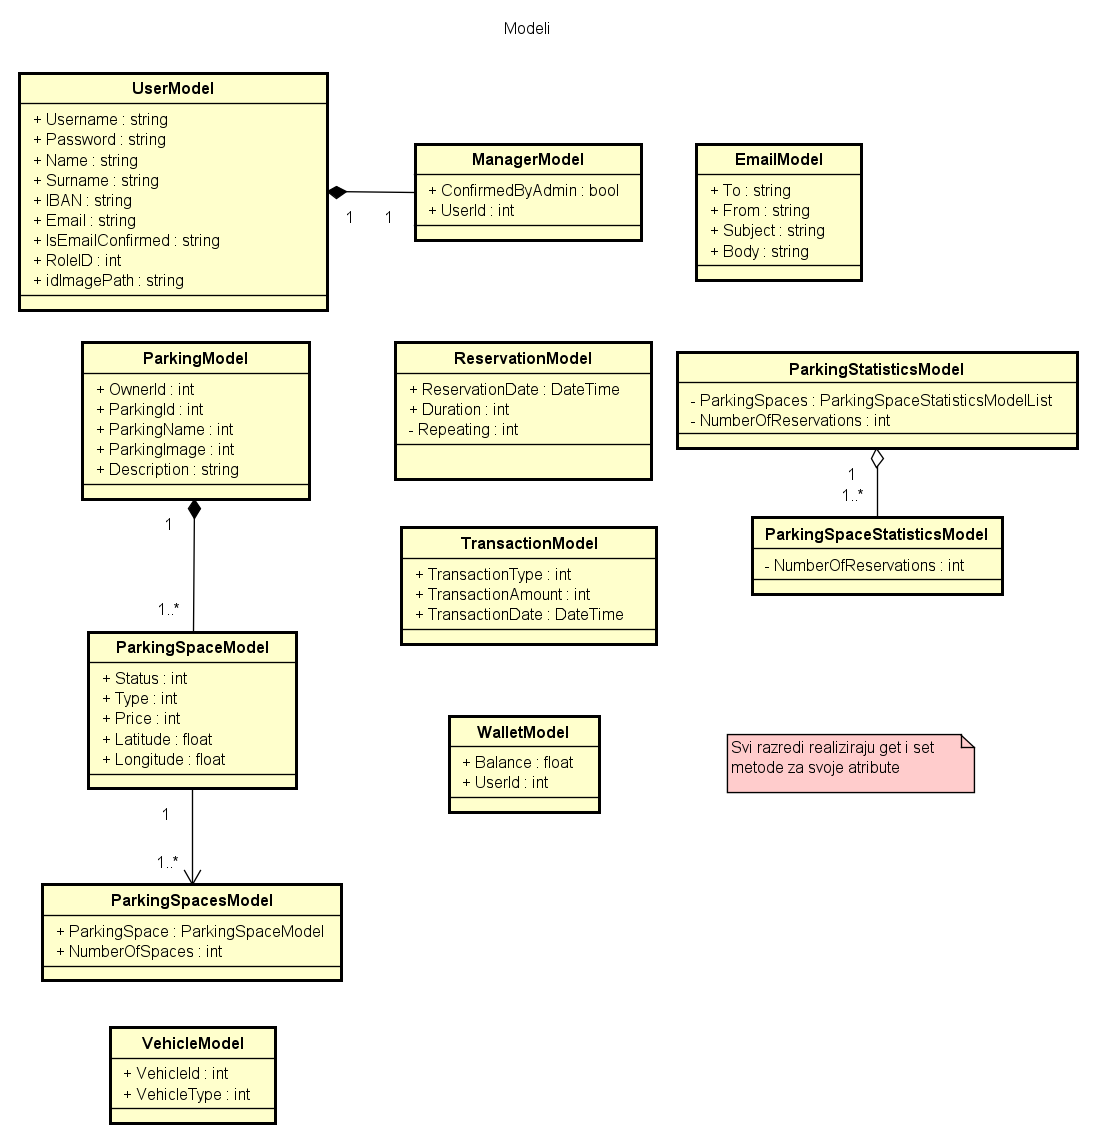
\includegraphics[width=\textwidth,keepaspectratio]{slike/progi_1.png}
				\caption{dio Models}
				\label{fig:models}
			\end{figure}
			\eject
		
			
			\begin{figure}[h]
				\centering
				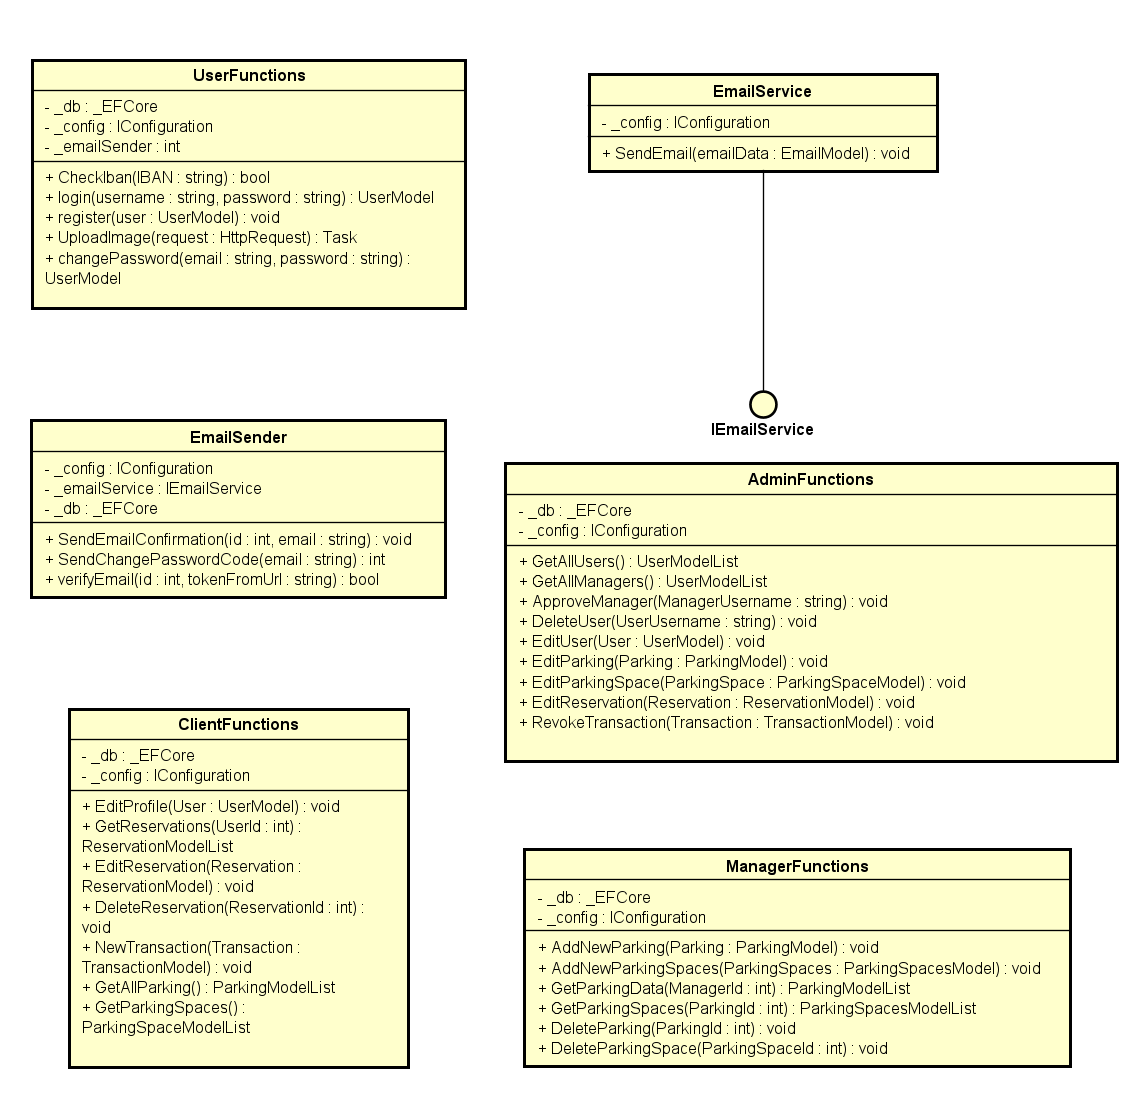
\includegraphics[width=\textwidth,keepaspectratio]{slike/progi3_1.png}
				\caption{dio Services}
				\label{fig:services}
			\end{figure}
			
			{U dijagramu razreda na slici \ref{fig:services} prikazani je dio servisa. Svi servisi kao svoj atribut, između ostalih, imaju instancu objekta \_EFCore koji predstavlja kontekst za bazu podataka i instancu IConfiguration objekta koji služi za dohvaćanje konstanti. Funkcije definirane u pojedinom razredu dohvaćaju, mijenjaju i dodaju podatke u bazu podataka i manipuliraju podacima koje vraćaju kontroleru koji šalje nazad do korisnika.}
			
			\begin{figure}[h]
				\centering
				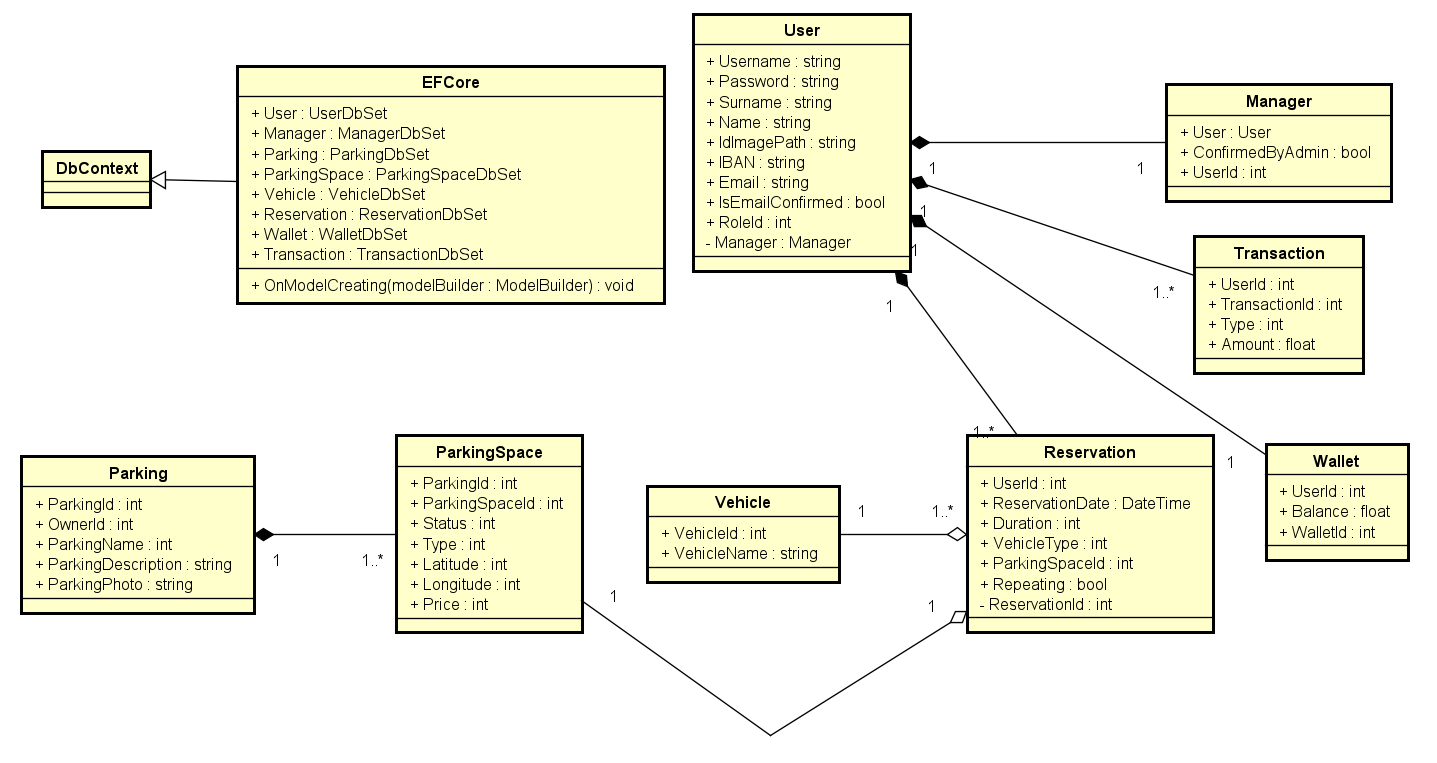
\includegraphics[width=\textwidth,keepaspectratio]{slike/progi2_1.png}
				\caption{Reprezentacija baze podataka}
				\label{fig:repr}
			\end{figure}
			
			\eject
			
			\pagebreak
		
		\section{Dijagram stanja}
			
			\textbf{\textit{dio 2. revizije}}\\
			
			\textit{Potrebno je priložiti dijagram stanja i opisati ga. Dovoljan je jedan dijagram stanja koji prikazuje \textbf{značajan dio funkcionalnosti} sustava. Na primjer, stanja korisničkog sučelja i tijek korištenja neke ključne funkcionalnosti jesu značajan dio sustava, a registracija i prijava nisu. }
			
			
			\eject 
		
		\section{Dijagram aktivnosti}
			
			\textbf{\textit{dio 2. revizije}}\\
			
			 \textit{Potrebno je priložiti dijagram aktivnosti s pripadajućim opisom. Dijagram aktivnosti treba prikazivati značajan dio sustava.}
			
			\eject
		\section{Dijagram komponenti}
		
			\textbf{\textit{dio 2. revizije}}\\
		
			 \textit{Potrebno je priložiti dijagram komponenti s pripadajućim opisom. Dijagram komponenti treba prikazivati strukturu cijele aplikacije.}